\vspace{-0.2cm}
\subsection{Analysis: Uncertainty Calibration in Offline Model-Based RL}
\label{sec:uq}
\vspace{-0.2cm}

\begin{figure}[t]
    \vspace{-0.5cm}
        \centering
        % 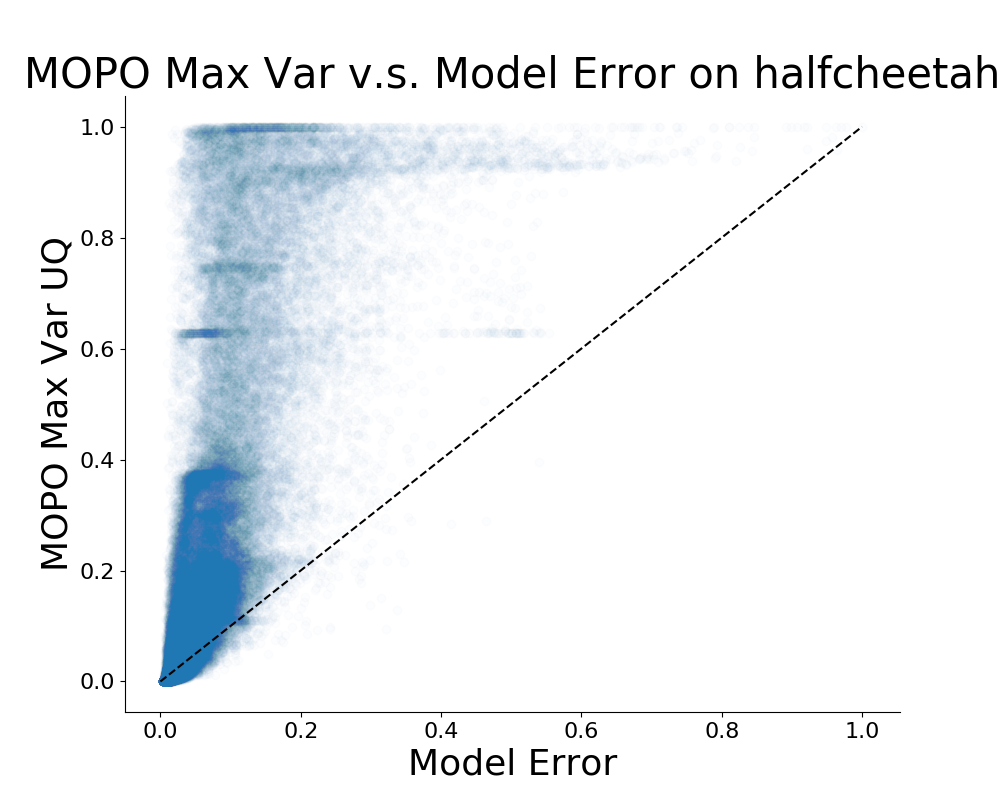
\includegraphics[width=0.47\linewidth]{halfcheetah_medium_corr_var_ood.png}
        % 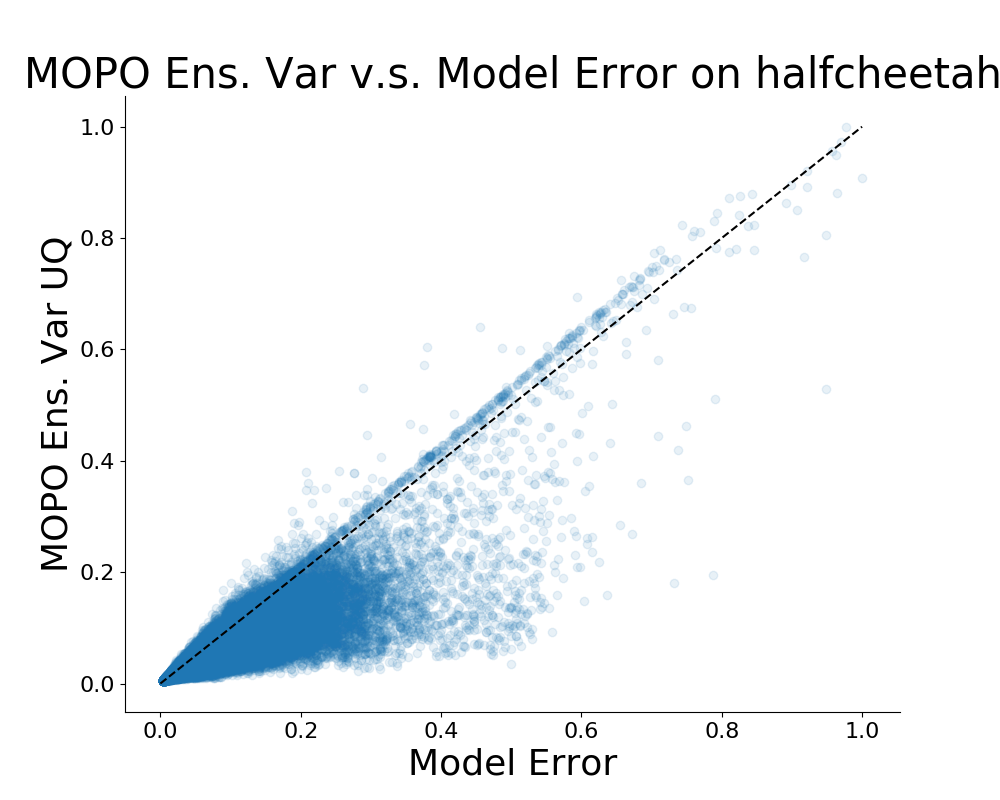
\includegraphics[width=0.47\linewidth]{halfcheetah_medium_corr_lip_ens_ood.png}
        % 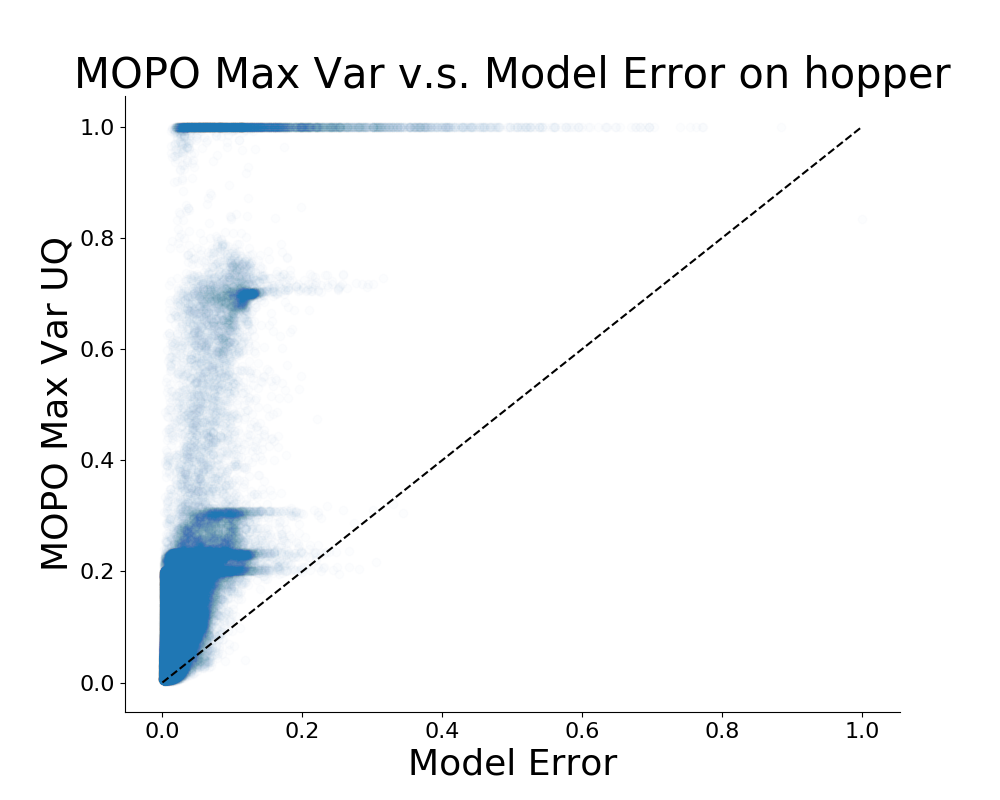
\includegraphics[width=0.47\linewidth]{hopper_medium_corr_var_ood.png}
        % 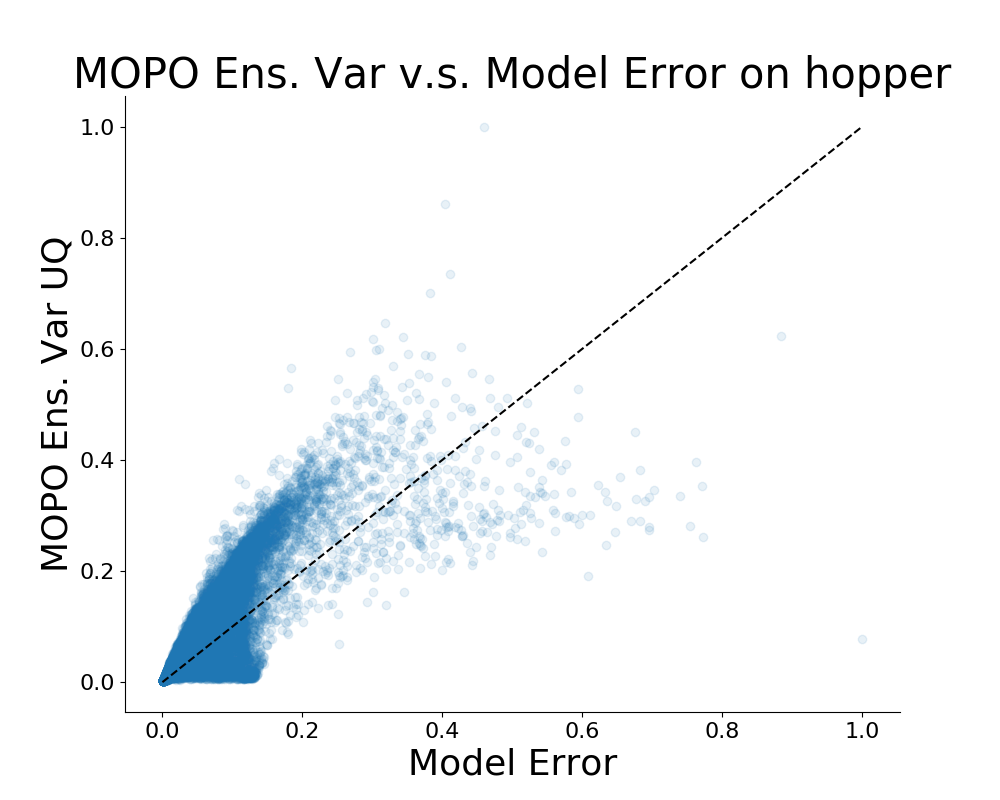
\includegraphics[width=0.47\linewidth]{hopper_medium_corr_lip_ens_ood.png}
        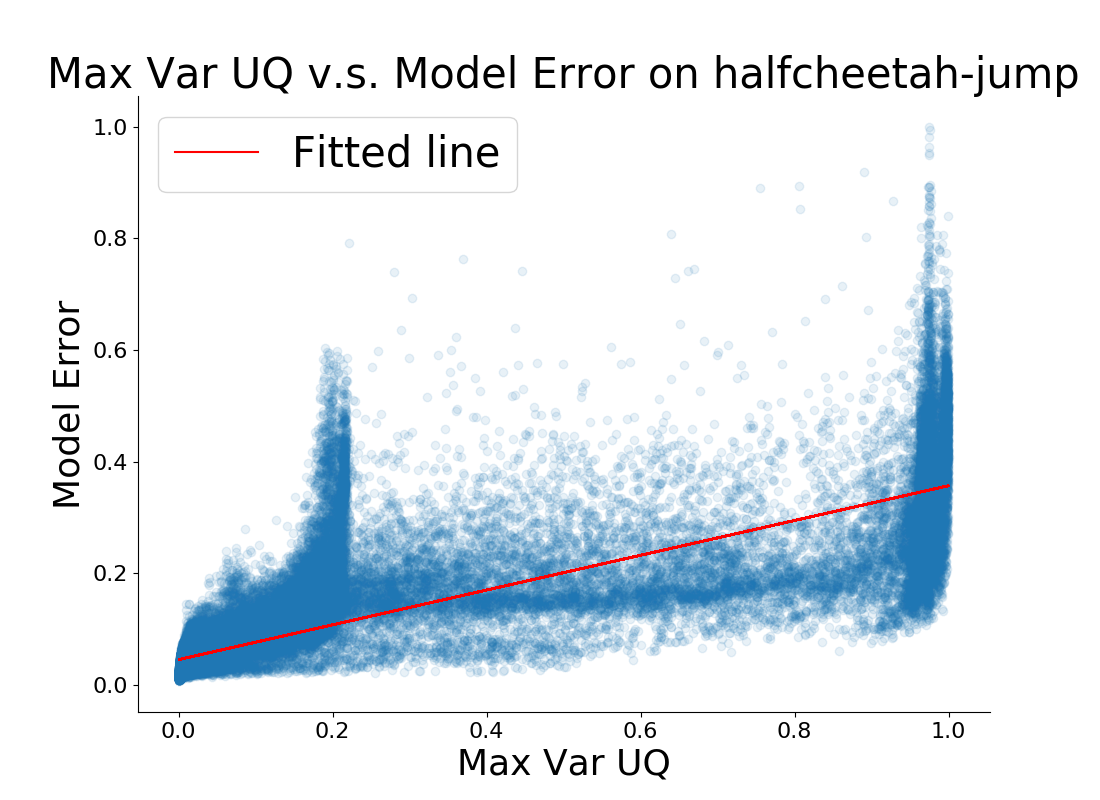
\includegraphics[width=0.45\textwidth]{chapters/combo/halfcheetah_jump_linear_regression_lip_ens_ood.png}
        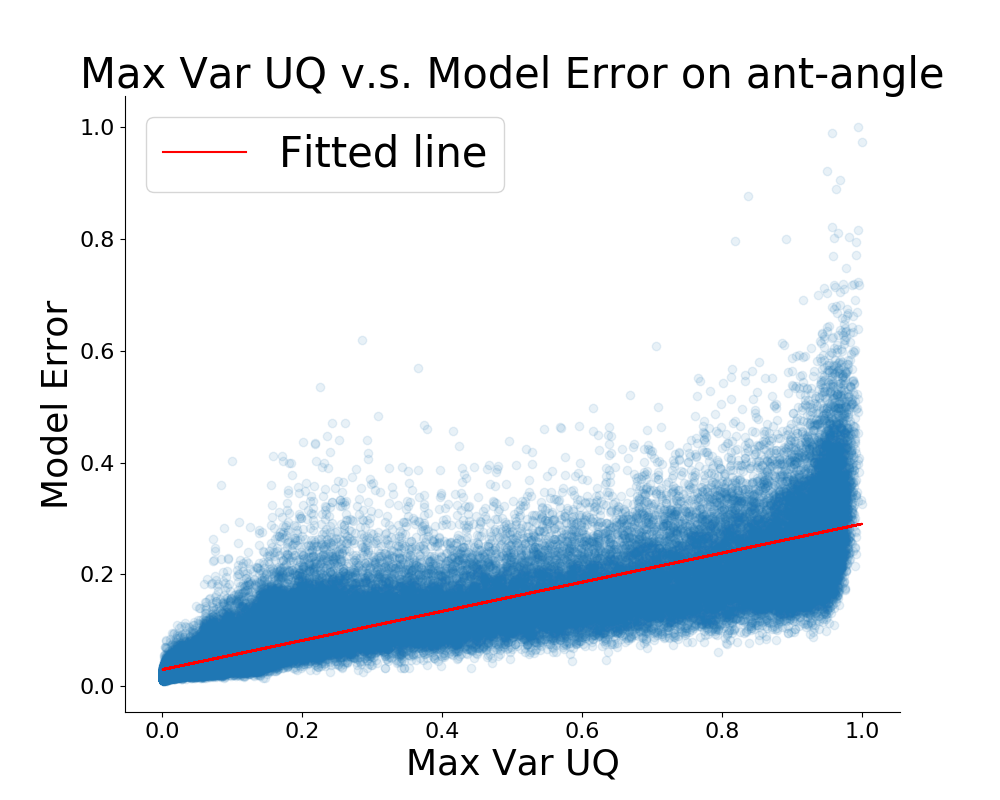
\includegraphics[width=0.41\textwidth]{chapters/combo/ant_angle_linear_regression_lip_ens_ood.png}
        \vspace{-0.2cm}
        \caption{\footnotesize {We visualize the fitted linear regression line between the model error and two uncertainty quantification methods maximum learned variance over the ensemble (denoted as \textbf{Max Var}) on two tasks that test the generalization abilities of offline RL algorithms (\texttt{halfcheetah-jump} and \texttt{ant-angle}). We show that \textbf{Max Var} struggles to predict the true model error. Such visualizations indicates that uncertainty quantification is challenging with deep neural networks and could lead to poor performance in model-based offline RL in settings where out-of-distribution generalization is needed. In the meantime, COMBO addresses this issue by removing the burden of performing uncertainty quantification.}}
        \label{fig:uq}
        \vspace{-0.4cm}
\end{figure}

In this section, we first analyze the efficacy of uncertainty estimation in existing model-based offline RL approaches. Specifically, we perform empirical evaluations to study whether uncertainty quantification with deep neural networks, especially in the setting of dynamics model learning, is challenging and could cause problems with uncertainty-based model-based offline RL methods such as MOReL~\citep{kidambi2020morel} and MOPO~\citep{yu2020mopo}. We pick tasks where the underlying model-based offline RL method is required to produce policies that need to go further away from the data distribution to obtain good performance. In our evaluations, we consider maximum learned variance over the ensemble (denoted as \textbf{Max Var}) $\max_{i=1,\dots,N}\|\Sigma^i_\theta(\bs, \mathbf{a})\|_\text{F}$ (used in MOPO).

We consider two tasks \texttt{halfcheetah-jump} and \texttt{ant-angle} (more details about the task in Appendix~\ref{app:ood_details}). We normalize both the model prediction error and the uncertainty estimates to be within scale $[0, 1]$ and performs linear regression that learns the mapping between the uncertainty estimates and the true model error. As shown in Figure~\ref{fig:uq}, on both tasks, \textbf{Max Var} is unable to accurately predict the true model error, suggesting that uncertainty estimation used by offline model-based methods is not accurate and might be the major factor that results in its poor performance. On the other hand, our approach, COMBO, alleviates the need for accurate uncertainty quantification by viewing model-based offline RL from the lens of conservative value function learning.

\vspace{-0.2cm}
\subsection{Conservative Offline Model-Based Policy Optimization}
\label{sec:combo}
\vspace{-0.2cm}
 
Our goal in this section is to develop a model-based offline RL algorithm that enables optimizing a lower bound on the policy performance, but without requiring uncertainty quantification. We achieve this by extending conservative Q-learning, from the previous section, into the model-based setting. Our algorithm, summarized in Algorithm~\ref{alg:combo}, alternates between a conservative policy evaluation step and a policy improvement step, which we outline below.

{\bf Conservative Policy Evaluation:} Given a policy $\policy$, an offline dataset $\data$, and a learned model of the MDP $\mhat$, the goal in this step is to obtain a conservative estimate of $Q^\policy$. To achieve this, we penalize the Q-values evaluated on data drawn from a particular state-action distribution that is more likely to be out-of-support while pushing up the Q-values on state-action pairs that are trustworthy, which is implemented by repeating the following recursion:

\begin{small}
\begin{align}
    \min_{Q} \beta\left(\E_{\bs, \mathbf{a} \sim \rho(\bs,\mathbf{a})}\!\left[Q(\bs,\mathbf{a})\right]-\E_{\bs, \mathbf{a} \sim \data}\left[Q(\bs,\mathbf{a})\right]\right) + \frac{1}{2}\E_{\bs, \mathbf{a}, \bs' \sim d_f}\left[ \left(Q(\bs, \mathbf{a}) - \widehat{\bellman}^\policy\hat{Q}^k(\bs, \mathbf{a}))\right)^2 \right].
    \label{eq:implicit_update}
\end{align}
\end{small}

Here, $\rho(\bs, \mathbf{a})$ and $d_f$ are sampling distributions that we can choose. Model-based algorithms allow ample flexibility for these choices while providing the ability to control the bias introduced by these choices. For $\rho(\bs, \mathbf{a})$, we make the following choice:
\[
\rho(\bs, \mathbf{a}) =  d^\policy_{\mdphat} (\bs) \pi(\mathbf{a} | \bs),
\]
where $d^\policy_{\mdphat} (\bs)$ is the discounted marginal state distribution when executing $\policy$ in the learned model $\mdphat$. Samples from $d^\policy_{\mdphat} (\bs)$ can be obtained by rolling out $\policy$ in $\mdphat$.
Similarly, $d_f$ is an $f-$interpolation between the offline dataset and rollouts from the model:
\[
d_f^\mu (\bs, \mathbf{a}) := f \ d(\bs, \mathbf{a}) + (1-f) \ d^\mu_{\mdphat} (\bs, \mathbf{a}),
\]
where $f \in [0,1]$ is the ratio of the datapoints drawn from the offline dataset as defined in Section~\ref{sec:combo_prelim} and $\mu(\cdot | \bs)$ is the rollout distribution used with the model, which can be modeled as $\policy$ or a uniform distribution. For brevity, we also denote $d_f := d_f^\mu$.

Under such choices of $\rho$ and $d_f$, we push down Q-values on state-action tuples from model rollouts and push up Q-values on the real state-action pairs from the offline dataset. When updating Q-values with the Bellman backup, we use a mixture of both the model-generated data and the real data, similar to Dyna~\cite{sutton1991dyna}. 
Note that in comparison to CQL and other model-free algorithms, COMBO learns the Q-function over a richer set of states beyond the states in the offline dataset. 
This is made possible by performing rollouts under the learned dynamics model, denoted by $d^\mu_{\mdphat} (\bs, \mathbf{a})$.
We will show in Section~\ref{sec:combo_theory} that the Q function learned by repeating the recursion in Equation~\ref{eq:implicit_update} provides a lower bound on the true Q function, without the need for explicit uncertainty estimation. Furthermore, we will theoretically study the advantages of using synthetic data from the learned model, and characterize the impacts of model bias.

\begin{algorithm}[t!]
\begin{small}
  \caption{COMBO: Conservative Model Based Offline Policy Optimization}\label{alg:combo}
  \begin{algorithmic}[1]
    \Require Offline dataset $\data$, rollout distribution $\mu(\cdot|\bs)$, learned dynamics model $\widehat{T}_\theta$, initialized policy and critic  $\policy_\phi$ and $Q_\psi$.
    \State Train the probabilistic dynamics model $\widehat{T}_\theta(\bs', r|\bs,\mathbf{a}) = \mathcal{N}(\mu_\theta(\bs, \mathbf{a}), \Sigma_\theta(\bs, \mathbf{a}))$ on $\data$.
    \State Initialize the replay buffer $\data_{\text{model}} \leftarrow \varnothing$.
    \For{$i=1, 2, 3, \cdots,$}
    \State Perform rollouts by drawing samples from $\mu$ and $\widehat{T}_\theta$ starting from states in $\data$. Add model rollouts to $\data_\text{model}$.
    \State Conservatively evaluate the policy by solving eq.~\ref{eq:implicit_update} to obtain $\hat{Q}^{\policy_\phi^i}_\psi$ using data sampled from $\data \cup \data_\text{model}$.
    \State Improve policy under state marginal of $d_f$ by solving eq.~\ref{eq:combo_policy_improvement} to obtain $\policy_\phi^{i+1}$.
    \EndFor
  \end{algorithmic}
\end{small}
\end{algorithm}

{\bf Policy improvement using a conservative critic:} After learning a conservative critic $\hat{Q}^\policy$, we improve the policy as:
\begin{equation}
\label{eq:combo_policy_improvement}
\policy' \leftarrow \arg \max_{\policy} \ \mathbb{E}_{\bs \sim \rho, \mathbf{a} \sim \policy(\cdot|\bs)} \left[ \hat{Q}^{\policy} (\bs, \mathbf{a}) \right]
\end{equation}
where $\rho(\bs)$ is the state marginal of $\rho(\bs,\mathbf{a})$. When policies are parameterized with neural networks, we approximate the $\arg \max$ with a few steps of gradient descent. In addition, entropy regularization can also be used to prevent the policy from becoming degenerate if required~\cite{haarnoja2018soft}. In Section~\ref{sec:policy_improvement_theory}, we show that the resulting policy is guaranteed to improve over the behavior policy.

\textbf{Practical implementation details.} Our practical implementation largely follows MOPO, with the key exception that we perform conservative policy evaluation as outlined in this section, rather than using uncertainty-based reward penalties. Following MOPO, we represent the probabilistic dynamics model using a neural network, with parameters $\theta$, that produces a Gaussian distribution over the next state and reward: $\widehat{T}_\theta(\bs_{t+1}, r| \bs, \mathbf{a}) = \mathcal{N}(\mu_\theta(\bs_t, \mathbf{a}_t), \Sigma_\theta(\bs_t, \mathbf{a}_t))$. The model is trained via maximum likelihood. For training the conservative critic, which is the major distinction between COMBO and MOPO, the fixed constant $\beta$ is tuned with an offline cross-validation scheme for all low-dimensional continuous control tasks and is decided with a limited number of rollouts in the actual environment in the vision-based environments. We set the ratio $f = 0.5$ to have an equal split between model rollouts and data from the offline dataset. For conservative policy evaluation (eq.~\ref{eq:implicit_update}) and policy improvement (eq.~\ref{eq:combo_policy_improvement}), we augment $\rho$ with states sampled from the offline dataset, which shows more stable improvement in practice. Additional details about practical implementation are provided in Appendix~\ref{app:combo_details}.

\vspace{-0.2cm}
\subsection{Theoretical Analysis of COMBO}
\label{sec:combo_theory}
\vspace{-0.2cm}
In this section, we theoretically analyze a simplified variant of COMBO and show that, like CQL, it continues to optimize a lower-bound on the expected return of the learned policy. The specific simplification we consider is a Bellman backup operator that considers a mixture of the model-free and model-based Bellman backup operator, with a weight $f$. The lower bound for COMBO that we show is close to the actual policy performance (modulo sampling error) when the policy's state-action marginal distribution is in support of the state-action marginal of the behavior policy and conservatively estimates the performance of a policy otherwise. By optimizing the policy against this lower bound, COMBO guarantees policy improvement beyond the behavior policy. {Furthermore, we use these insights to discuss cases when COMBO is less conservative compared to CQL}.

\vspace{-0.2cm}
\subsubsection{COMBO Optimizes a Lower Bound}
\label{sec:combo_lower_bound}
\vspace{-0.2cm}
We first show that training the Q-function using Equation~\ref{eq:implicit_update} produces a Q-function such that the expected off-policy policy improvement objective~\citep{degris2012off} computed using this learned Q-function lower-bounds its actual value. We will reuse notation for $d_f$ and $d$ from Section~\ref{sec:combo}. 
% With a slight abuse of notation, we will assume that $d_f$ and $\data$ denote (empirical) distributions over the state-action space.
%%TY.1.31: it's a bit unclear what D_f is. In Section 4, it is currently defined as the interpolation, but here it seems to refer to an arbitrary state-action distribution.
Assuming that the Q-function is tabular, the Q-function found by approximate dynamic programming in iteration $k$, can be obtained by differentiating Equation~\ref{eq:implicit_update} with respect to $Q^k$ (see App.~\ref{app:combo_proofs} for details):
\begin{equation}
    \hat{Q}^{k+1}(\bs, \mathbf{a}) = (\widehat{\mathcal{B}}^\pi Q^k)(\bs, \mathbf{a}) - \beta \frac{\rho(\bs, \mathbf{a}) - d(\bs, \mathbf{a})}{d_f(\bs, \mathbf{a})}.
\label{eqn:combo_iterate}
\end{equation}
Equation~\ref{eqn:combo_iterate} effectively applies a penalty that depends on the three distributions appearing in the COMBO critic training objective (Equation~\ref{eq:implicit_update}), of which $\rho$ and $d_f$ are free variables that we choose in practice as discussed in Section~\ref{sec:combo}. For a given iteration $k$ of Equation~\ref{eqn:combo_iterate}, we further define the expected penalty under $\rho(\bs, \mathbf{a})$ as: 
\begin{equation}
 \nu(\rho, f) := \E_{\bs, \mathbf{a} \sim \rho(\bs, \mathbf{a})}\left[\frac{\rho(\bs, \mathbf{a}) - d(\bs, \mathbf{a})}{d_f(\bs, \mathbf{a})} \right]\label{eqn:expected_penalty}.
\end{equation}
% Before stating our main result, we will first show that the penalty term in Equation~\ref{eqn:combo_iterate} is positive in expectation. Such a positive penalty is important to combat any overestimation that may arise as a result of using $\bellmanhat$. 

% \begin{lemma}[Interpolation Lemma]
% \label{thm:line_thm}
% For any $f \in [0, 1]$, and any given $\rho(\bs, \mathbf{a}) \in \Delta^{|\states||\actions|}$, let $d_f$ be an f-interpolation of $\rho$ and $\data$, i.e., $d_f(\bs, \mathbf{a}) := f d(\bs, \mathbf{a}) + (1-f) \rho(\bs, \mathbf{a})$. For a given iteration $k$ of Equation~\ref{eqn:combo_iterate}, define the expected penalty under $\rho(\bs, \mathbf{a})$ as: 
% \begin{equation*}
%  \nu(\rho, f) := \E_{\rho}\left[\frac{\rho(\bs, \mathbf{a}) - d(\bs, \mathbf{a})}{d_f(\bs, \mathbf{a})} \right].
% \end{equation*}
% Then $\nu(\rho, f)$ satisfies, (1) $\nu(\rho, f) \geq 0,~~ \forall \rho, f$, (2) $\nu(\rho, f)$ is monotonically increasing in $f$ for a fixed $\rho$, and (3) $\nu(\rho, f) = 0$ iff $\forall~ \bs, \mathbf{a}, ~\rho(\bs, \mathbf{a}) = d(\bs, \mathbf{a}) \text{~or~} f = 0$. 
% \end{lemma}
% The proof can be found in Appendix~\ref{app:proof_lemma}.
% Lemma~\ref{thm:line_thm} characterizes $\rho(\bs, \mathbf{a})$ for which COMBO (Equation~\ref{eq:implicit_update}) induces a conservative penalty. 
% COMBO sets $\rho(\bs) = d^\pi_{\mdphat}(\bs)$ 
% %%SL.1.31: Nitpick: you defined D_f(s,a) before, not D_f(s). While it's easy to guess what D_f(s) is, it is undefined
% and uses $\rho(\mathbf{a}|\bs) = \pi(\mathbf{a}|\bs)$, and hence each step of update (Equation~\ref{eqn:combo_iterate}) penalizes the Q-function making it more conservative. The total amount of conservatism induced in the Q-function, given by $\nu(\rho, f)$, is controlled by the choice of $f$. Based on result (2) in Lemma~\ref{thm:line_thm}, we note that by controlling the amount of real data, $f$, we can control the amount of conservatism: $f=1$ induces the maximum conservatism, and $f=0$ induces no conservatism at all.

% Next, we will show that the asymptotic Q-function learned by COMBO lower-bounds the actual Q-function of any policy $\pi$ with high probability for a large enough $\beta \geq 0$. Let $\mdpbar$ represent the empirical MDP which uses the empirical transition model based on raw data counts. The Bellman backups over the dataset distribution $d_f$ in equation~\ref{eq:implicit_update} can be interpreted as an $f-$interpolation 
% of the backup operator in the empirical MDP (denoted by $\bellman_{\mdpbar}^\pi$) and the backup operator under the learned model $\mdphat$ (denoted by $\bellman_{\mdphat}^\pi$).
% The empirical backup operator suffers from sampling error, but is unbiased in expectation, whereas the model backup operator induces bias but no sampling error.
% We assume that all of these backups enjoy concentration properties with concentration coefficient $C_{r, T, \delta}$, dependent on the desired confidence value $\delta$ (details in Appendix~\ref{app:proof_lower_bound}). This is a standard assumption in literature~\citep{laroche2019safe}.
% Now, we state our main results below.

% \begin{proposition}[Asymptotic lower-bound]
% \label{thm:Q_bound}
% Let $P^\pi$ denote the Hadamard product of the dynamics $P$ and a given policy $\pi$ in the actual MDP and let $S^\pi := (I - \gamma P^\pi)^{-1} c_{S}$, where $c_{S}$ is a suitably chosen positive constant. Let $D$ denote the total-variation divergence between two probability distributions. For any $\pi(\mathbf{a}|\bs)$, the Q-function obtained by recursively applying Equation~\ref{eqn:combo_iterate}, with $\hat{{\bellman}}^\pi = f \bellman_{\mdpbar}^\pi + (1 - f) \bellman_{\mdphat}^\pi$, with probability at least $1 - \delta$, results in $\hat{Q}^\pi$ that satisfies:
% \begin{align*}
%     \forall \bs, \mathbf{a},~ \hat{Q}^\pi(\bs, \mathbf{a}) \leq  Q^\pi(\bs, \mathbf{a}) - \beta \cdot \epsilon_{\text{c}} + f \epsilon_{\text{s}} + (1 - f)\epsilon_{\text{m}},
% \end{align*}
% where vector forms of $\epsilon_{\text{s}}$, $\epsilon_{\text{c}}$ and $\epsilon_{\text{m}}$ are given by:
% %%CF: Is there a reason why you chose this order? It would be more intuititve for me to have the order match the order that they appear in the inequality above.
% \small{
% \begin{align*}
%     \epsilon_{\text{c}} := \left[ \frac{1}{c_S} S^\pi \left[ \frac{\rho - d}{d_f} \right] \right], \epsilon_{\text{m}} := \left[ S^\pi \left[ |R - R_{\mdphat}| \!+\! \frac{ 2 \gamma  R_{\max}}{1 - \gamma} D(P, P_{\mdphat}) \right]  \right],~ \epsilon_{\text{s}} &:= \left[ S^\pi \left[ \frac{C_{r, T, \delta} R_{\max}}{(1 - \gamma) \sqrt{|\data|}} \right] \right].
%     %%CF: Has the distance D been defined?
% \end{align*}
% }
% \end{proposition}
% The proof for Proposition~\ref{thm:Q_bound} can be found in Appendix~\ref{app:proof_lower_bound}. 

Next, we will show that the Q-function learned by COMBO lower-bounds the actual Q-function under the initial state distribution $\mu_0$ and any policy $\pi$. We also show that the asymptotic Q-function learned by COMBO lower-bounds the actual Q-function of any policy $\pi$ with high probability for a large enough $\beta \geq 0$, which we include in Appendix~\ref{app:proof_lower_bound}. Let $\mdpbar$ represent the empirical MDP which uses the empirical transition model based on raw data counts. The Bellman backups over the dataset distribution $d_f$ in equation~\ref{eq:implicit_update} can be interpreted as an $f-$interpolation 
of the backup operator in the empirical MDP (denoted by $\bellman_{\mdpbar}^\pi$) and the backup operator under the learned model $\mdphat$ (denoted by $\bellman_{\mdphat}^\pi$).
The empirical backup operator suffers from sampling error, but is unbiased in expectation, whereas the model backup operator induces bias but no sampling error.
We assume that all of these backups enjoy concentration properties with concentration coefficient $C_{r, T, \delta}$, dependent on the desired confidence value $\delta$ (details in Appendix~\ref{app:proof_lower_bound}). This is a standard assumption in literature~\citep{laroche2019safe}.
Now, we state our main results below.
\begin{theorem}
\label{thm:lower_bound}
For large enough $\beta$, we have
$\E_{\bs \sim \mu_0, \mathbf{a} \sim \policy(\cdot|\bs)}[\hat{Q}^\pi(\bs, \mathbf{a})] \leq \E_{\bs \sim \mu_0, \mathbf{a} \sim \policy(\cdot|\bs)}[Q^\pi(\bs, \mathbf{a})]$, 
where $\mu_0(\bs)$ is the initial state distribution. 
Furthermore, when $\epsilon_{\text{s}}$ is small, such as in the large sample regime, or when the model bias $\epsilon_{\text{m}}$ is small, a small $\beta$ is sufficient to guarantee this condition along with an appropriate choice of $f$.
\end{theorem}
%%SL.5.24: Could we explain a bit more intuitively what the significance of a small beta being sufficient is?

The proof for Theorem~\ref{thm:lower_bound} can be found in Appendix~\ref{app:proof_lower_bound}.
% Corollary~\ref{thm:lower_bound} directly appeals to Proposition~\ref{thm:Q_bound} and Lemma~\ref{thm:line_thm}.
% Proposition~\ref{thm:Q_bound} further implies that for large $\beta$,
%%CF: I think you mean "for large beta" or "for non-zero beta" here?
% deviating away from the behavior policy is expected to lead to smaller values.
Finally, while \citet{kumar2020conservative} also analyze how regularized value function training can provide lower bounds on the value function at each state in the dataset~\citep{kumar2020conservative} (Proposition 3.1-3.2), \textit{our result shows that COMBO is less conservative in that it does not underestimate the value function at every state in the dataset like CQL (Remark~\ref{remak:tighter_lower_bound})} and might even overestimate these values. Instead COMBO penalizes Q-values at states generated via model rollouts from $\rho(\bs, \mathbf{a})$. While it is challenging to argue that that either COMBO or CQL attains the tightest possible lower-bound on return, in our final result of this section, we discuss a sufficient condition for the COMBO lower-bound to be tighter than CQL. 

\begin{tcolorbox}[colback=blue!6!white,colframe=black,boxsep=0pt,top=3pt,bottom=5pt]
\begin{theorem}[CQL vs COMBO]
%%CF.5.25: can we give a name to this? (like was done for 4.1)
\label{prop:less_conservative}
Let $\Delta^\pi_{\text{COMBO}} := \E_{\bs, \mathbf{a} \sim d_{\mdpbar}(\bs), \pi(\mathbf{a}|\bs)}\left[ \hat{Q}^\pi(\bs, \mathbf{a}) \right]$ and $\Delta^\pi_{\text{CQL}} := \E_{\bs, \mathbf{a} \sim d_{\mdpbar}(\bs), \pi(\mathbf{a}|\bs)}\left[ \hat{Q}^\pi_\text{CQL}(\bs, \mathbf{a}) \right]$ denote the average values on the dataset under the Q-functions learned by COMBO and CQL respectively. 
%%CF.5.25: put notation outside of the Proposition statement?
Then, $\Delta^\pi_{\text{COMBO}} \geq \Delta^\pi_\text{CQL}$, if:
\begin{equation*}
    \E_{\bs, \mathbf{a} \sim \rho(\bs,\mathbf{a})}\left[ \frac{\pi(\mathbf{a}|\bs)}{\behavior(\mathbf{a}|\bs)} \right] - \E_{\bs, \mathbf{a} \sim d_{\mdpbar}(\bs), \pi(\mathbf{a}|\bs)}\left[ \frac{\pi(\mathbf{a}|\bs)}{\behavior(\mathbf{a}|\bs)} \right] \leq 0.~~~~~~~~~~~(*)
    % \sum_{\bs, \mathbf{a}} \left(\rho(\bs) - d_{\mdpbar}(\bs)\right) \frac{\pi^2(\mathbf{a}|\bs)}{\behavior(\mathbf{a}|\bs)} \leq 0.~~~~~~~~~~~(*)
\end{equation*}
\end{theorem}
\end{tcolorbox}
Proposition~\ref{prop:less_conservative} indicates that COMBO will be less conservative than CQL when the action probabilities under learned policy $\pi(\mathbf{a}|\bs)$ and the probabilities under the behavior policy $\pi_\beta(\mathbf{a}|\bs)$ are closer together on state-action tuples drawn from $\rho(\bs, \mathbf{a})$ (i.e., sampled from the model using the policy $\pi(\mathbf{a}|\bs)$), than they are on states from the dataset and actions from the policy, $d_{\mdpbar}(\bs)\pi(\mathbf{a}|\bs)$.
%%SL.5.24: The above sentences are easy to misunderstand. Can we rephrase like this: when the action probabilities under learned policy $\pi(\mathbf{a}|\bs)$ and the probabilities under the behavior policy $\pi_\beta(\mathbf{a}|\bs)$ are closer together on state-action tuples drawn from $\rho(\bs, \mathbf{a})$ (i.e., sampled from the model using the policy $\pi(\mathbf{a}|\bs)$), than they are on states from the dataset and actions from the policy, $d_{\mdpbar}(\bs)\pi(\mathbf{a}|\bs)$. [that said, I'm not sure this intuition is quite right...]
COMBO's objective (Equation~\ref{eq:implicit_update}) only penalizes Q-values under $\rho(\bs, \mathbf{a})$, which, in practice, are expected to primarily consist of out-of-distribution states generated from model rollouts, and does not penalize the Q-value at states drawn from $d_{\mdpbar}(\bs)$. As a result, the expression $(*)$ is likely to be negative, making COMBO less conservative than CQL.
%%CF.5.25:  It would be really good to talk about what this means in combination with prop 4.1. In isolation, this result is of course not meaningful on its own. (i.e. lower-bound plus often less conservative means often closer to the actual Q-value. (unless I am misunderstanding something here)

%%SL.5.24: I'm not sure I follow this logic -- why should we expect it to be negative?
% COMBO does not underestimate the value function at every state in the dataset like \citet{kumar2020conservative}, but only lower-bounds the expected value function under the initial state distribution as discussed in Corollary~\ref{thm:lower_bound}. We elaborate on how COMBO is less conservative as it attains tighter lower bounds in Remark~\ref{remak:tighter_lower_bound} (Appendix~\ref{app:proof_lower_bound}).

\vspace{-0.2cm}
\subsubsection{Model-Based Safe Policy Improvement}
\label{sec:policy_improvement_theory}
\vspace{-0.2cm}

Now that we have shown various aspects of the lower-bound on the Q-function induced by COMBO, we provide policy improvement guarantees for the COMBO algorithm. As mentioned earlier, we consider a simplified variant for COMBO for this result, which utilizes a Bellman backup operator that interpolates between the model-based backup operator and model-free backup operator, with a weight equal to the fraction $f$. Formally, Proposition~\ref{thm:policy_improvement} discuss safe improvement guarantees over the behavior policy, building on prior work~\citep{laroche2017safe,kumar2020conservative}. 

\begin{tcolorbox}[colback=blue!6!white,colframe=black,boxsep=0pt,top=3pt,bottom=5pt]
\begin{theorem}[$\zeta$-safe policy improvement]
\label{thm:policy_improvement}
Let $\hat{\pi}_{\text{out}}(\mathbf{a}|\bs)$ be the policy obtained by COMBO. Then, the policy $\hat{\pi}_{\text{out}}(\mathbf{a}|\bs)$ is a $\zeta$-safe policy improvement over ${\behavior}$ in the actual MDP $\mdp$, i.e., $J(\hat{\pi}_{\text{out}}, \mdp) \geq J({\behavior}, \mdp) - \zeta$, with probability at least $1 - \delta$, where $\zeta$ is given by,
\small{
\begin{align*}
    \mathcal{O}\left(\frac{\gamma f}{(1 - \gamma)^2}\right) ~&\underbrace{\E_{\bs \sim d^{\hat{\pi}_{\text{out}}}_{\mdp}}\left[ \sqrt{\frac{|\actions|}{|\data(\bs)|} \mathrm{D}_{\text{CQL}}(\hat{\pi}_{\text{out}}, \behavior)} \right]}_{:=~ \text{(1)}}\\
    &+ \mathcal{O}\left(\frac{\gamma (1 - f)}{(1 - \gamma)^2}\right) \underbrace{ \mathrm{D_{TV}}(\mdpbar, \mdphat)}_{:=~ \text{(2)}} - \underbrace{\beta \frac{\nu(\rho^\pi, f) - \nu(\rho^\beta, f)}{(1 - \gamma)}}_{:=~ \text{(3)}}.
\end{align*}
}
\end{theorem}
\end{tcolorbox}

The complete statement (with constants and terms that grow smaller than quadratic in the horizon) and proof for Proposition~\ref{thm:policy_improvement} is provided in Appendix~\ref{app:proof_policy_improvement}. $D_{\text{CQL}}$ denotes a notion of probabilistic distance between policies~\citep{kumar2020conservative} which we discuss further in Appendix~\ref{app:proof_policy_improvement}. The expression for $\zeta$ in Proposition~\ref{thm:policy_improvement} consists of three terms: term (1)~captures the decrease in the policy performance due to limited data, and decays as the size of $\mathcal{D}$ increases. The second term (2)~captures the suboptimality induced by the bias in the learned model. Finally, as we show in Appendix~\ref{app:proof_policy_improvement}, the third term (3)~is equivalent to the improvement in policy performance as a result of running COMBO in the empirical and model MDPs. Since the learned model is trained on the dataset $\data$ with transitions generated from the behavior policy $\behavior$, the marginal distribution $\rho^\beta(\bs, \mathbf{a})$ is expected to be closer to $d(\bs, \mathbf{a})$ for $\behavior$ as compared to the counterpart for the learned policy, $\rho^\pi$. Thus, term (3) is expected to be positive in practice, and in such cases, an appropriate (large) choice of $\beta$ will make term (3) large enough to counteract terms (1) and (2) that reduce policy performance. We discuss this elaborately in Appendix~\ref{app:proof_policy_improvement} (Remark~\ref{remark:remark1}). 

Further note that in contrast to Proposition 3.6 in \citet{kumar2020conservative}, note that our result indicates the sampling error (term (1)) is reduced (multiplied by a fraction $f$) when a near-accurate model is used to augment data for training the Q-function, \neurips{and similarity, it can avoid the bias of model-based methods by relying more on the model-free component. This allows COMBO to attain the best-of-both model-free and model-based methods, via a suitable choice of the fraction $f$.}
% \textcolor{red}{[if the above stuff makes sense -- it is just setting model error and Q-function sampling error in a way so as to optimize for a non-zero f -- I can formally write it down. However the assumption is a bit adhoc -- it is unclear why model-bias is large when sampling error ir small, but we will have to assume this.]}
To summarize, through an appropriate choice of $f$, Proposition~\ref{thm:policy_improvement} guarantees safe improvement over the behavior policy without requiring access to an oracle uncertainty estimation algorithm.
% Proposition~\ref{thm:policy_improvement} only depends on an appropriate choice single, scalar $f \in [0, 1]$, which can be controlled in practice and gets rid of the strict requirement of oracle access to a uniformly-accurate uncertainty metric.   
%%CF: Can we put this in the opposite order to match the order in the previous sentences?

